\chapter{Introduction
    \pgsize{25 p.}
}
\label{chap:introduction}

In this thesis, we discuss how multiple artifacts of different tools to develop a software or software-intensive system can be kept consistent.
We research how multiple specifications for consistency and its preservation can be developed independently, such that their combination operates \emph{correctly} and such that they can be \emph{reused} modularly.



%%
%% MOTIVATION
%%
\section{Consistency of Multiple Models}

\mnote{System complexity is increasing}
Engineers develop software and software-intensive technical systems of ever increasing scale.
This leads to a continuous increase in complexity of the artifacts used to describe such systems~\cite{murer2011evolution}.
Engineers inevitably have to deal with the inherent essential complexity, as a direct consequence of the increasing system sizes.
Tools, however, are supposed to reduce accidental complexity to allow engineers to focus on handling the essential complexity~\cite{brooks1987NoSilverBullet-Computer, fraser2008NoSilverBulletReloaded-Software}.

\subsection{Consistency in System Engineering}

\mnote{Fragmented information to deal with essential complexity}
To better handle the essential complexity, engineers usually use multiple tools to describe and analyze different parts or properties of a system under development by different artifacts, in the following denoted as \emph{models}.
This reduces the information that different roles have to deal with to what is relevant for their development task.
In classical engineering disciplines like construction, mechanical and electrical engineering, this has been common practice for a long time and is often called \emph{\gls{MBSE}}~\cite{estefan2007MbseSurvey}.
For example, the development of \glspl{ECU} software in automobiles comprises different tools or standards for specifying the system and software architecture, such as SysML~\cite{sysml} or AUTOSAR~\cite{scheid2015autosar}, for defining the behavior, such as MATLAB/Simulink~\cite{simulink} or ASCET~\cite{ascet}, and for defining the deployment on multi-core hardware architectures, such as Amalthea~\cite{amalthea, wolff2014a}.
In software engineering, such a development methodology is also getting growing attention, often called \emph{\gls{MDSD}}~\cite{stahl2006a}.
Such a development process foresees other artifacts beyond code as primary artifacts to describe the system under construction.
While code only specifies the functionality of a systems, other tools can be used, for example, for defining the software architecture and its deployment, such as the \gls{UML}~\cite{uml}, analyzing and predicting the software performance, such as the Palladio Simulator~\cite{reussner2016a}, and for specifying the requirements, like IBM Rational Doors~\cite{laplante2012RequirementsEngineering-Book}.

\mnote{Information fragmentation increases accidental complexity}
While this \emph{fragmentation} of information across models in different tools eases dealing with the essential complexity of a system, it increases the accidental complexity.
Since all these models describe the same system, they usually share an overlap of information in terms of implicit \emph{dependencies} or \emph{redundancies}, which can lead to \emph{inconsistencies} if overlapping information is not modified properly across all dependencies and redundancies.
On a high level, for example, requirements changes have to be reflected in the software architecture and implementation, and modifications of the software architecture have to be reflected in the code.
Since systems are usually developed iteratively and incrementally, there is no strict direction in which changes have to be propagated to preserve consistency, but in general any model can be changed and require updates of others.

\mnote{Fragmented information needs to be kept consistent}
The overlaps of information, for example in the above mentioned tools for \gls{ECU} software development~\cite{giese2010a}, are often not documented explicitly~\cite{mazkatli2017ase}, but only known by engineers.
Performing the task of updating overlapping information manually is, however, time-consuming and error-prone.
The automation of checking and of preserving consistency of information is still poorly supported in current development processes for large systems, as a recent survey has shown \owncite{guissouma2018study}.
Automating that process is, however, necessary to reduce the accidental complexity induced by the fragmentation of information across multiple models.

\mnote{State of research: transformations to preserve consistency}
A common approach to automate the process of checking and preserving consistency of models are \emph{model transformations}.
If models shall or cannot be generated anew after each change, especially \emph{incremental} transformations are of interest.
Such transformation specify how models have to updated after engineers make changes  to one or some of them instead of generating new models.
Especially \emph{bidirectional} model transformations~\cite{stevens2010sosym}, which specify the relations between two models and routines how consistency of their instances can be restored after changes in any of them, are well researched.
System development usually involves more than two tools and thus more than two models to be kept consistent.
The use of transformations to check and preserve consistency between more than two models is, however, less researched~\cite{stevens2020BidirectionalTransformationLarge-SoSym}.
It gained recent attention by a dedicated Dagstuhl seminar~\cite{cleve2019dagstuhl}.


\subsection{Modular and Independent Consistency Specification}

\mnote{Multidrectional transformations vs. networks}
Two general approaches for consistency of multiple, especially more than two, models by means of transformations are \emph{multidirectional} transformations or the combination of multiple transformations to networks of them.
A single multidirectional transformations is beneficial from a theoretical perspective, because it is not prone to contradictions between the transformations to combine and it provides higher expressiveness~\cite{stevens2020BidirectionalTransformationLarge-SoSym}.
For practical application, however, multidirectional transformations suffer from missing modularity, requiring a single person or team to define the overall relations between all tools.
It is, however, difficult to think about complex n-ary relations~\cite{stevens2020BidirectionalTransformationLarge-SoSym} and, even worse, the knowledge necessary to define such a relation may not even exist~\owncite{klare2018docsym}.

\begin{figure}
    \centering
    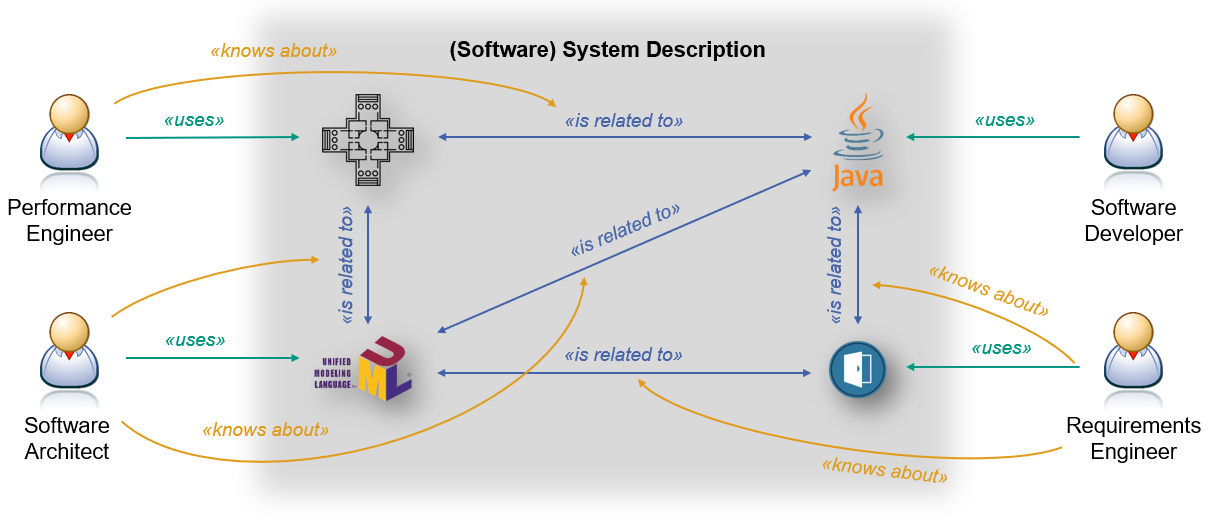
\includegraphics[width=\textwidth]{figures/prologue/distributed_knowledge.png}
    \caption[Tools and distributed knowledge in engineering processes]{Different tools and roles involved in an exemplary software development process and distributed knowledge about the relations between models of the different tools}
    \label{fig:prologue:distributedknowledge}
\end{figure}

\mnote{Distributed knowledge about consistency}
Domain experts deal with the tools and corresponding models they require for their tasks in developing a system.
Usually, each of them is only concerned with a subset of all tools involved in the development of a system.
For example, a performance engineer may be concerned with an instance of the \gls{PCM}, which represents a component-based architecture description of the system, to perform an architecture-based prediction of the system's performance and knows how this description is reflected in the system implementation in Java.
A software architect may use \gls{UML} models for the architecture specification and know how they are related to the implementation as well as to the component-based performance models in \gls{PCM}.
Finally, a requirements engineer may use IBM Rational Doors and know how they have to be reflected in the architecture specification and implementation to consider the models consistent.
These exemplary relations are depicted in \autoref{fig:prologue:distributedknowledge}.
No matter whether this is how knowledge is actually present at the different roles in a concrete scenario, it emphasizes that knowledge about the relations between tools and their models will usually be distributed across different experts as soon as there are several models involved.
In large software systems, a single developer cannot know about all model dependencies~\cite{petrenko2008a}.
In consequence, a process for specifying consistency by means of transformation has to support a kind of \emph{modularity} to foster independent specification of distributed knowledge.
% Maybe discuss that not only binary is case if covered, but also modular multiary case

\mnote{Reuse of consistency specifications}
Furthermore, an automation especially proposes benefits if it is used often.
A specification of consistency and its preservation between common tools, for example, \gls{UML} and a programming language such as Java, can be reused across multiple projects.
Not each project, however, will use exactly the same tools.
Considering the example in \autoref{fig:prologue:distributedknowledge}, if the relation between \gls{PCM} and Java was partly expressed indirectly across \gls{UML}, it would not be possible to reuse that specification in another project that only uses \gls{PCM} and Java but omits \gls{UML}.
Thus parts of specifications, i.e., specification between subsets of the tools in a project, should be reusable, comparable to \gls{COTS}.
In consequence, a process for specifying consistency by means of transformations has to support \emph{independence} of the modular specifications, such that they can be reused without the others.

\mnote{Context assumptions}
To support the context induced by the previous considerations, we focus on combinations of transformations, be they binary or n-ary, instead of having only a single n-ary transformations.
We call such a combination a \emph{transformation network}.
To summarize the previous considerations, we need to cover the following context assumptions to the specification of the individual transformations of a network:
\begin{description}
    \item[Modularity:] Transformations are defined in a modular way, i.e., each transformation does only the specification of consistency and its preservation between a subset of the tools used for a development project.
    \item[Independence:] Transformations are defined independently, i.e., each transformation can be developed without considering the contents of the other transformations to be combined with.
\end{description}


\subsection{Orchestration of Transformation Networks}

\mnote{Limitations of transformation orchestration strategies}
Combining several modular and independently developed transformations requires their \emph{orchestration}, i.e., the decision which of the transformations are executed in which order to restore consistency.
Existing work proposes, for example, to define an execution order explicitly ~\cite{pilgrim2008a, vanhooff2007UniTI-MODELS} or to derive a kind of topologic order~\cite{stevens2020BidirectionalTransformationLarge-SoSym}.
Such approaches either require a manual decision for the orchestration or restrict the execution to specific topologies, such as a directed acyclic graph or tree, which limits the kinds of supported transformation networks.
In any case, severe assumptions to the individual transformations or the network topology are made.
%To foster distributed development and partial reuse, arbitrary topologies should be supported (Universality, Reusability).

\mnote{Research gap: universal combination of specifications}
It is yet unclear, how arbitrary modular and independently developed transformations can be combined in a universal way.
%This especially concerns the role of the transformation developer.
It is neither known how a developer can achieve a \emph{correct} transformation network specification, i.e., transformations and an orchestration of them that delivers consistent models when applied, nor how he or she can improve quality attributes of the network such as %\emph{reusability} and 
\emph{comprehensibility}.
%For the role of the transformation user, it is yet unknow how to support him in understanding the reasons whenever transformations fail to deliver consistent models.

%\mnote{Two roles: transformation users and developers}
%Fragmentation addresses challenges of transformations users.
%Challenges of developers yet addressed for binary case.

\begin{figure}
    \centering
    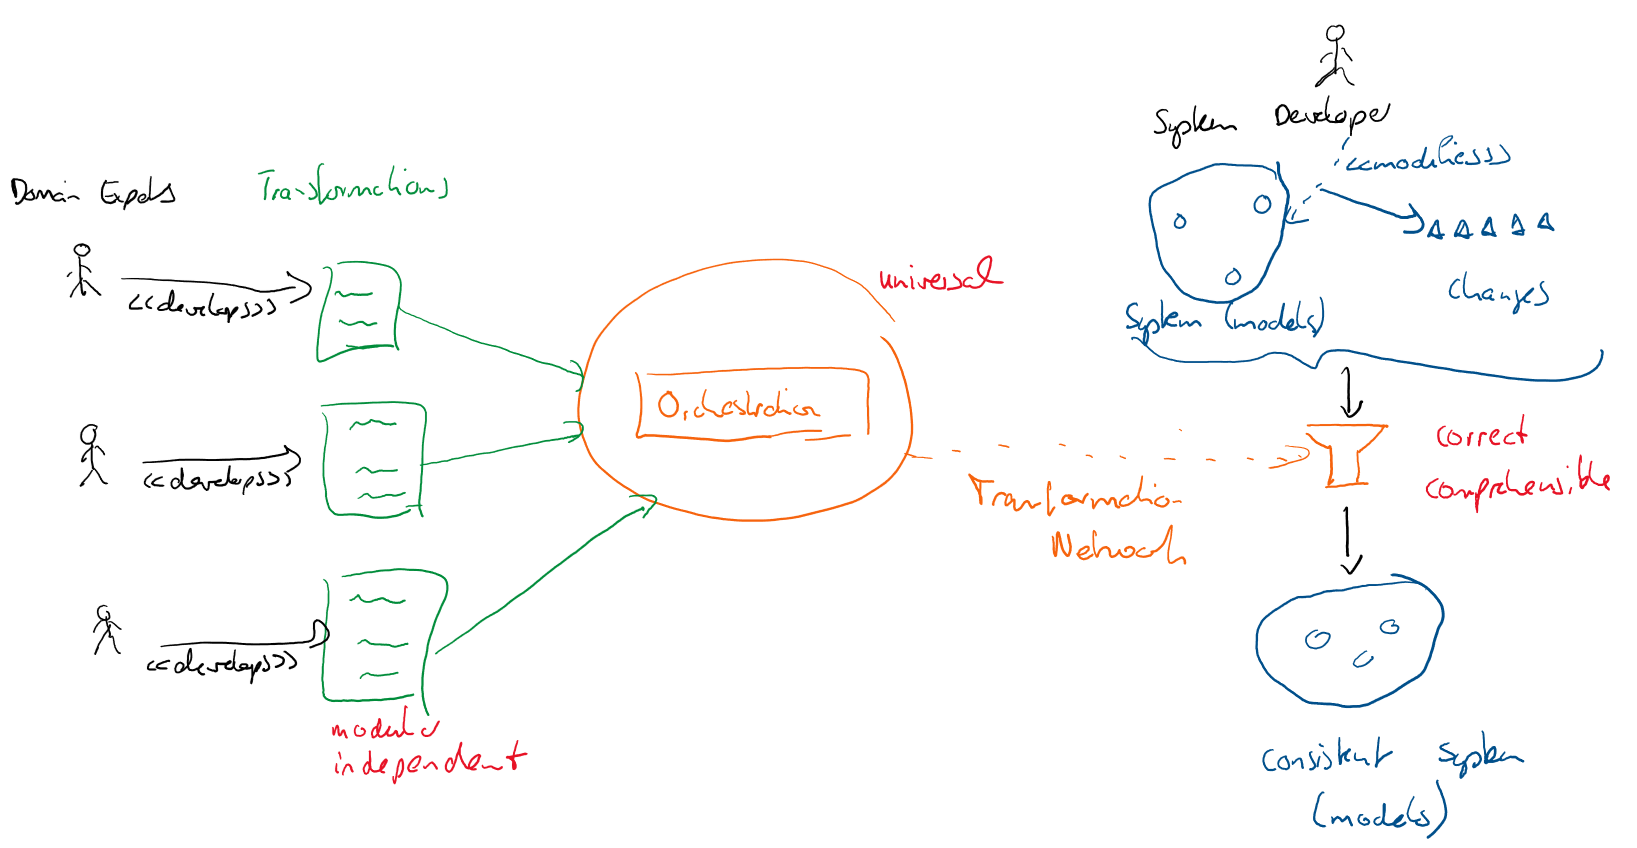
\includegraphics[width=\textwidth]{figures/prologue/overall_process.png}
    \caption[Process of specifying and executing a transformation network]{The process of specifying and executing a transformation network. Different domain experts specify transformations, which are combined to a transformation network by an orchestration mechanism that decides which transformations have to be executed in which order. If an actual system is developed and a developer modified models, the network is applied to these models and the performed changes to produce a consistent system description again. Artifacts defined by transformation developers are marked green, artifacts at runtime are marked blue and the artifacts for orchestration and application developed in this thesis are marked orange. The assumed and envisioned properties are denoted in red.}
    \label{fig:prologue:processoverview}
\end{figure}

\mnote{Envisioned properties and process}
Under the assumption of a modular and independent specification of the individual transformation, we aim at an approach for executing transformation networks that have the following properties:
\begin{description}
    \item[Universality:] The approach shall be able to process transformation networks of arbitrary topology. Especially to support the assumption of independent development, there should be no restriction regarding specific kinds of topologies to be supported.
    %It must be possible to combine arbitrary specifications. This means that the approach should not restrict which specifications can be combined, especially not which topology, induced by the specifications (such as only a tree) should be supported. In fact, requirements that all specifications have to fulfill may be defined, but apart from that the usability of one specification should not depend on the existence or non-existence of another.
    \item[Correctness:] The approach shall operate correctly. If the approach applies transformations to preserve consistency of models, the result must be consistent or indicate an error.
    %\item[Reusability:] The approach shall improve reusability. This means that the individual transformations shall be reusable independently.
    \item[Comprehensibility:] The approach shall improve comprehensibility. If the transformations are not able to produce models that are actually consistent, it should support the user in finding the reason for that.
\end{description}
The envisioned process and artifacts as well as the required properties are depicted in \autoref{fig:prologue:processoverview}.
\todo{Maybe add non-intrusiveness?}

\mnote{Thesis contributions}
In this thesis, we contribute to support the process of building transformation networks that have the defined properties by providing a formal foundation for transformation networks of arbitrary topology and defining a formal notion of correctness for them.
We discuss how correctness of a universal approach to orchestrate and apply the transformations of a network network can be achieved by construction or at least by analysis, and which properties the different involved artifacts, such as transformations and their orchestration, have to fulfill for that.
The proposed strategy to orchestrate transformations improves comprehensibility in cases when it is not able to execute transformations such that they deliver consistent models.
Additionally, we classify which kinds of errors can occur when the artifacts are not defined correctly.
We also analyze how topologies of networks affect the desired properties and propose an approach of defining transformations that resolves trade-offs between the envisioned properties.

\mnote{Towards a detailed problem statement}
In the following, we first discuss the addressed problem in more detail by considering a specific scenario and generalizing some of the problems to give a first impression of the issues we have to address.
Afterwards, we derive our general research goal and define several questions arising from that.
After more precisely specifying the context and assumptions that we make, we give a detailed overview of our contributions.



%%
%% PROBLEM DESCRIPTION -> RESEARCH GAP
%%
\section{Consistency Specification Challenges}

To get an impression of problems arising from the combination of modular transformations, we introduce an exemplary scenario from a software engineering process.
We motivate why we expect the necessity to have multiple executions of the same transformations and discuss some of the issues that can occur in that context.
Afterwards, we generalize that scenario and derive a more precise problem statement.

\mnote{Software engineering scenario}
Let us consider an extract of a software engineering scenario, in which three roles using three different tools are involved, according to \autoref{fig:prologue:distributedknowledge}. 
A software developers implements the system with an object-oriented programming language such as Java.
An architect manages the object-oriented architecture of the system with \gls{UML}. 
Finally, a performance engineer uses a component-based representation of the architecture with the \gls{PCM} containing an abstract behavior description at the architecture level to predict the system's performance and help to evaluate different design decisions.

\mnote{Contents of \gls{PCM}}
In \gls{PCM}, the basic entities are components, interfaces and datatypes.
Components are units of reuse that define which interfaces they provide or require and contain abstract service specifications for the operations of the interfaces they provide.
This allows to assemble a systems of components by connecting components through their interfaces, such that every required interface of one component is provided by a defined other component.
For the consistency relations between the three languages \gls{PCM}, \gls{UML} and Java, we use the ones proposed by \textcite{langhammer2017a} between \gls{PCM} and object-oriented design, be it \gls{UML} or Java, and the intuitive notion of consistency between \gls{UML} and Java.

\begin{figure}
    \centering
    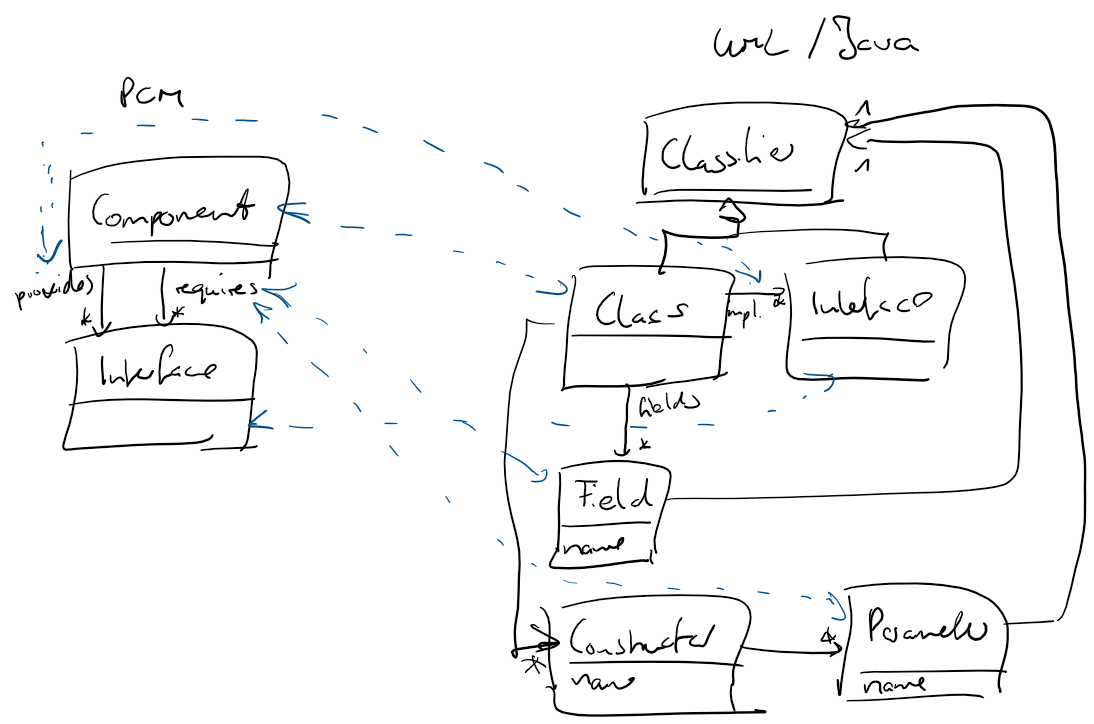
\includegraphics[width=\textwidth]{figures/prologue/scenario_consistency_relations.png}
    \caption[Consistency relation for \acrshort{PCM} and \gls{UML}/Java]{Extract of consistency relations between a component-based architecture description in \gls{PCM} and the object-oriented design in \gls{UML}/Java according to \cite{langhammer2017a}.}
    \label{fig:prologue:scenario_consistency_relations}
\end{figure}

\mnote{Consistency relations between \gls{PCM}, \gls{UML} and Java}
Although there are several degrees of freedom to relate \gls{UML} and Java, the extracts that we consider follow a simple one-to-one mapping.
The relevant relations between \gls{PCM} and object-oriented design are depicted in \autoref{fig:prologue:scenario_consistency_relations}.
This involves a one-to-one mapping between interfaces and the realization of \gls{PCM} components as classes. 
Provided interfaces in \gls{PCM} are realized by interface implementations. 
Required interfaces are realized by a field with the type of the interface and constructor parameters that ensure that the required interfaces are set on instantiation of the component.

%% CORRECTNESS
\subsection{Correctness of Transformation Networks}

The central goal of (software) engineering, and thus also the construction of transformation networks as part of the engineering process, is to achieve \emph{correctness}.

\subsubsection*{Orchestration Challenge}

% 1. Orchestration problem
\mnote{Most changes require each transformation to be executed once}
When we consider transformations between \gls{PCM} and \gls{UML}, as well as between \gls{UML} and Java, they may transfer each modification to the other model.
For example, adding a \gls{PCM} component creates a class in \gls{UML}, which then creates a class in Java.
Although in most cases each transformation only needs to be executed once to propagate the information to all other models, there can be situations that require transformation to be executed repeatedly.

\begin{figure}
    \centering
    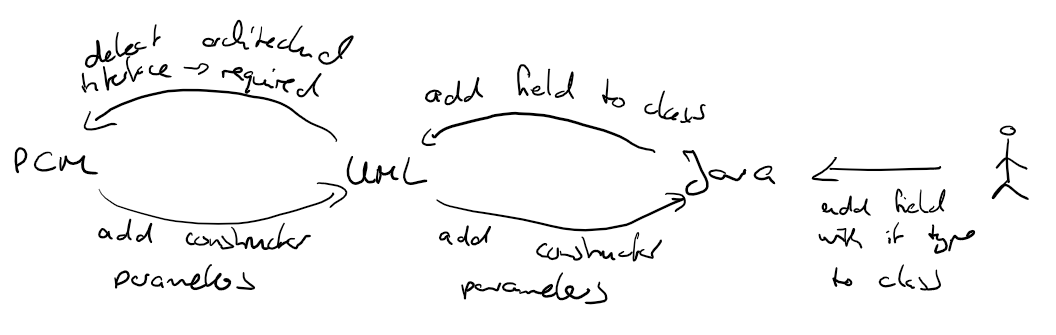
\includegraphics[width=\textwidth]{figures/prologue/scenario_duplicate_execution.png}
    \caption[Example for transformation orchestration]{Duplicate transformation execution after adding a field representing a required interface to a Java class.}
    \label{fig:prologue:scenario_duplicate_execution}
\end{figure}

\mnote{Scenario with multiple execution of same transformation}
In the process depicted in \autoref{fig:prologue:scenario_duplicate_execution}, we assume a system description that contains at least one component and class, respectively, and one interface.
If a developer adds a field to the Java class having the type of the interface, the transformation between \gls{UML} and Java transfers this field to the corresponding \gls{UML} class.
The transformation between \gls{UML} and \gls{PCM} detects that the interface is also represented as an architectural interface in the \gls{PCM} model, thus the field is supposed to represent a required interface in the architectural model.
In consequence, the transformation adds a required interface to the \gls{PCM} component.
Since the consistency relations prescribe each required interface to be represented as a constructor parameter, the transformation also adds a constructor parameter to the class in the \gls{UML} model.
This finally requires the transformation between \gls{UML} and Java to be executed again, since the Java code does not yet contain the constructor parameter introduced by the transformation between \gls{PCM} and \gls{UML}.

\mnote{Orchestration challenge}
The example demonstrates that, in general, it is necessary to execute each transformation in a network more than once to achieve a consistent state of the models.
This is always the case if at least two transformations modify the same model, because then the first transformation may need to react the changes of second one again, like in the example to transformation between \gls{UML} and Java needs to react to the one between \gls{PCM} and \gls{UML}, because both modified the \gls{UML} model.
The determination how often and in which order transformations have to be executed is what we call the \emph{orchestration challenge}.

\subsubsection*{Synchronization Challenge}
% 2. Synchronization problem
\mnote{Transformation between \gls{PCM} and Java}
We yet considered that we only have a chain of two transformations, one between \gls{PCM} and \gls{UML} and another between \gls{UML} and Java.
There may, however, also be an overlap of information between \gls{PCM} and Java that cannot be represented in \gls{UML}, which require to also define a transformation between \gls{PCM} and Java.
This is especially the case for behavioral properties, which cannot be expressed in UML class models, for example, the functionality defined by Java method implementations and the abstract service specifications in \gls{PCM}.
In consequence, the graph induced by the transformation contains a cycle.

\mnote{Transformation may contain redundancies}
Instead of only having a transformation for that overlapping information of \gls{PCM} and Java that cannot be expressed across \gls{UML}, the transformation may also contain the relations already expressed across \gls{UML}.
The reasons for that can be independent development and reusability.
Independent development leads to the situation that the developer of the transformation between \gls{PCM} and Java does not know what the transformations to \gls{UML} already express.
So even if the developer has that information, he may want to express it again to foster reusability, i.e., to use the transformation between \gls{PCM} and Java in projects in which no \gls{UML} is used or when the transformation is not supposed for a specific network of transformations, comparable to \gls{COTS}.
In consequence, we need to face the situation that multiple transformations propagate the same information, i.e., they contain redundancies.

\begin{figure}
    \centering
    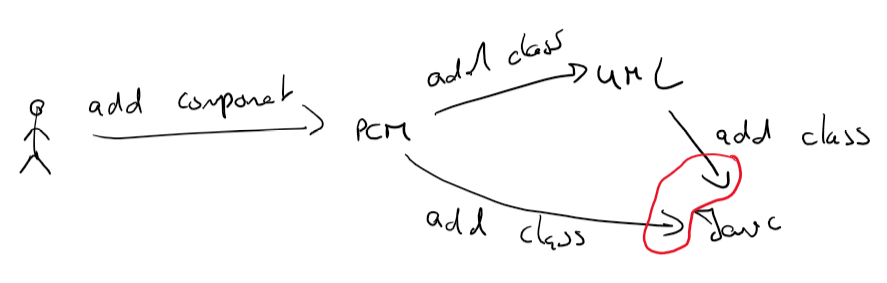
\includegraphics[width=\textwidth]{figures/prologue/scenario_synchronization.png}
    \caption[Example for transformation synchronization]{Two transformations propagating the same information to Java.}
    \label{fig:prologue:scenario_synchronization}
\end{figure}

\mnote{Two transformation paths for Java class creation}
\autoref{fig:prologue:scenario_synchronization} depicts a scenario, in which a user creates a \gls{PCM} component.
The transformations, in consequence, create a \gls{UML} class and finally, both the transformation between \gls{UML} and Java and the one between \gls{PCM} and Java define the creation of an appropriate Java class.
These transformation now have to consider that there may be another transformation that already created that class.
Otherwise, there is the risk of creating a duplicate of that class or of overwriting the already created on.

\mnote{Synchronization challenge}
Such a problem can always occur if two sequences of transformations propagate the same information to the same model, like here to Java.
In consequence, transformations have to properly deal with that case.
We call this the \emph{synchronization challenge}.

\subsubsection*{Contradiction Challenge}
% 3. Contradiction problem

\mnote{Equivalence of redundancies}
We have seen that it may be necessary to redundantly define the same consistency relations in different transformations.
We have, however, implicitly assumed that these repetitions of the same relations are true redundancies, i.e., express the relations equally.
This, in turn, requires all developers to have the same \emph{notion of consistency} between the languages.

\begin{figure}
    \centering
    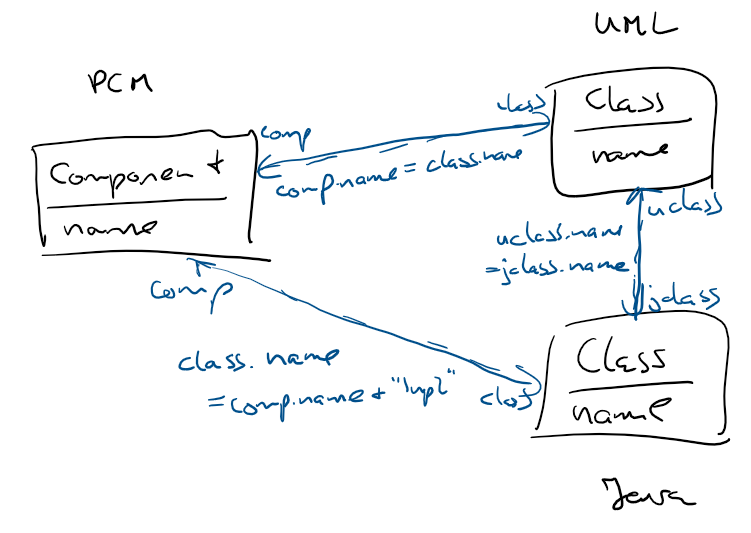
\includegraphics[width=0.6\textwidth]{figures/prologue/scenario_contradiction.png}
    \caption[Example for transformation contradictions]{Contradicting consistency relations between components in \gls{PCM} and classes in \gls{UML} and Java.}
    \label{fig:prologue:scenario_contradiction}
\end{figure}

\mnote{Contradicting component and class name relations}
The example in \autoref{fig:prologue:scenario_contradiction} informally depicts exemplary specifications for the relation between components and classes.
It is supposed to express that for each a component or class appropriate elements in the other models have to exist with the given name relation.
The constraints for their names can, however, obviously not be fulfilled at the same time.
While the class representations are supposed to have the same name and the \gls{PCM} is also supposed to have the same name as the \gls{UML} class, it is supposed to have the name of the Java class with an \enquote{Impl} suffix, as proposed by \textcite{langhammer2017a}.

\mnote{Differnt notions of consistency}
Such a situation can occur if the developers of the different transformations have different notions of consistency.
In this case, the performance engineering, who knows about the relation between \gls{PCM} and Java according to the scenario presented in \autoref{fig:prologue:distributedknowledge}, and the software architect, who knows about the relation between \gls{PCM} and \gls{UML} as well as between \gls{UML} and Java have different notions about how to represent components in object-oriented design.

\mnote{Non-terminate or inconsistent termination due to contradictions}
If the experts encode the defined relations in transformations that try to preserve them and execute them after any of the elements is added to a model, the transformations will either terminate in an inconsistent state or never terminate at all.
Executing the transformation for a finite number of times would always result in an inconsistent state, if not removing the element just added by the user.

\mnote{Contradiction challenge}
In consequence, it is important to avoid or detect situations in which transformations with such contradicting constraints are combined to a network.
We call this the \emph{contradiction challenge}

\subsubsection*{Problem Statement}

\mnote{No systematic knowledge on correctness issues}
We have discussed three kinds of issues, which can prohibit that a transformation network terminates consistently, and derived according challenges: orchestration, synchronization and contradiction.
These challenges only exemplify the relevant correctness issues in transformation networks. 
In fact, it is even not systematically known which issues can occur.
Thus we derive the following general problem statement:

\begin{problemstatement}
    It is unknown how to correctly combine modular and independently developed transformations to networks to achieve consistent results.
\end{problemstatement}

%% QUALITY PROPERTIES
\subsection{Quality of Transformation Networks}

\mnote{Quality properties of networks}
Like in ordinary (software) engineering, besides the primary goal of producing \emph{correct} artifacts, there are several quality properties that need to be improved.
They can range from properties relevant for developers, such as reusability and evolvability, to properties relevant for users, such as performance, scalability and reliability.
This similarly applies to transformation networks as artifacts of the (software) engineering process.

\subsubsection*{Properties and Topology Challenge}

\mnote{Focus on development properties}
In this thesis, we will focus on further properties regarding the development of a transformation network, such as reusability and evolvability, rather than properties of its usage, such as scalability.
Reusability is of most importance, because transformation may be used in different contexts within different networks of other transformations.

\begin{figure}
    \centering
    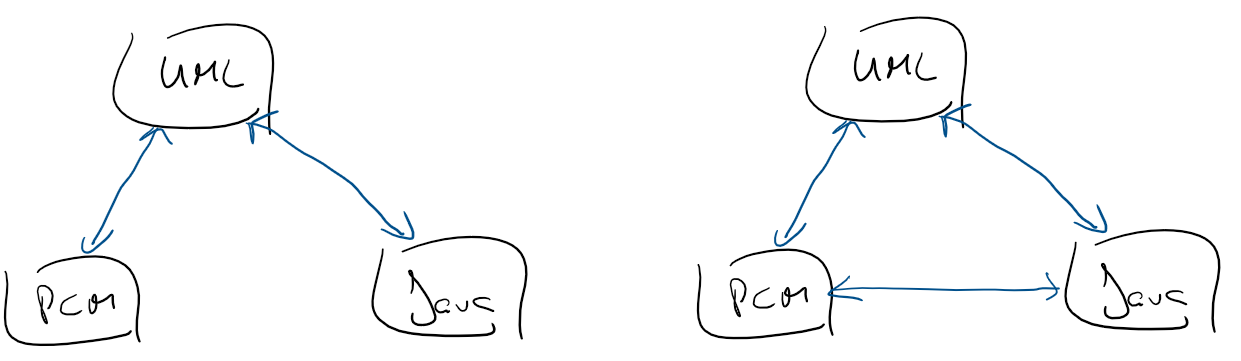
\includegraphics[width=\textwidth]{figures/prologue/scenario_topologies.png}
    \caption[Example for network topologies]{Different topologies of transformation networks for \gls{PCM}, \gls{UML} and Java}
    \label{fig:prologue:scenario_topologies}
\end{figure}

\mnote{Topology extremes: tree and dense graphs}
Consider the two networks depicted in \autoref{fig:prologue:scenario_topologies}.
The networks contain transformation between \gls{PCM} and \gls{UML} as well as between \gls{UML} and Java. 
One of them additionally contains a transformation between \gls{PCM} and Java.
They can be considered as representatives of extremes of transformation networks:
the graph induced by transformations may on the one end be a tree, and on the other be a dense graph.

\mnote{Topologies affect properties}
It is easy to see that properties are directly affected by the network topology.
A dense graph has to benefit of high reusability, because any subset of languages can be used for a development project without loosing consistency.
In the example, the tree network is not applicable in development projects using \gls{UML}, because then \gls{PCM} and Java cannot be kept consistent.
Additionally, a dense graph profits from universality, because arbitrary relations can be expressed, whereas a tree requires that of three language there is always one that can express the overlap of the two others.
If there are overlaps between \gls{PCM} and Java that cannot be expressed across \gls{UML}, like discussed for behavioral specifications, a tree cannot be defined.
On the other hand, a tree has the benefit of inherent correctness guarantees.
There are no two paths of transformations between the same two language.
Thus, no changes cab be propagated across two paths to the same model, avoiding synchronization problems, and no contradictions can occur.
This already avoids two of the three introduced challenges regarding correctness.

\mnote{Topologies induce trade-offs}
While each topology improves certain properties, it degrades others at the same time.
In other words, topologies induce trade-offs between different properties.
For example, a tree improved correctness, but degrades reusability in comparison to a dense graph.
Finding out how to use this knowledge to mitigate trade-offs and improve different properties at the same time is our \emph{properties and topologies challenge}.

\subsubsection*{Language Challenge}

\mnote{Language support for specific topology}
We have seen that topologies directly influence properties of a transformation network.
We will see that with an appropriate strategy of building networks with a specific topology, we can mitigate trade-offs.
Currently, however, there is no known approach that supports building transformation networks of specific topologies.
Research approaches did consider approaches and languages for single transformations or for specific composition purposes, such as transformations between the same two languages~\cite{wagelaar2010a,wagelaar2011a}, or chains of transformations~\cite{pilgrim2008a, vanhooff2007UniTI-MODELS}.

\mnote{Language challenge}
To relieve the developer from the task of following the strategy to a network of transformations to improve different properties, a suited language should be provided.
Finding how such a language should be designed constitutes our \emph{language challenge}.

\subsubsection*{Integration Challenge}

\mnote{Transformations assume models of specific formalisms}
Finally, we always assumed that models are developed and thus present in a format to which transformations can be applied.
Transformation languages have to assume a specific formalism of the languages between they transform~\cite{klare2017models}, thus the models have to follow that formalism.
This is especially problematic for code, which will be relevant for almost every development project.
Although there are tools that wrap code in a specific formalism, such as JaMoPP~\cite{heidenreich2009a,heidenreich2010a} for using Java code in the Eclipse Modeling Framework, recognizing incremental updates of code are still poorly supported.

\mnote{Models are often implicit}
Models are often contained implicitly in code.
This mostly concerns domain models for the software to be developed, but also models of code, such as the Java code representation in the Java Development Tools of the Eclipse Framework~\cite{EclipseJDT}, which has capabilities of recognizing incremental updates.

\mnote{Lifting artifacts to models}
Lifting such implicit models into a format according to formalisms that allow the application of transformations and transformation languages enables projects using such artifacts to apply transformation techniques to preserve consistency.
For all projects containing such artifacts, this can be seen as a preliminary for applying transformation network, as otherwise only the parts of the projects present in an appropriate formalism can be kept consistent.
In consequence, it can be seen as a \emph{completeness} property of the network.
We denote this as the \emph{integration challenge}.

\subsubsection*{Problem Statement}

\mnote{Impact of topologies and usability for mitigating trade-offs unknown}
We have discussed that topologies affect different correctness and quality properties of transformation network and that they impose trade-offs between them.
It is unclear how that insight can be used to systematically improve different properties by building transformation networks of specific topologies.
Thus we derive the following problem statement:

\begin{problemstatement}
    It is unknown how to systematically mitigate trade-off decisions between correctness and quality properties, such as reusability and evolvability, of transformation networks.
\end{problemstatement}


\subsection{Challenges Overview}

\begin{figure}
    \centering
    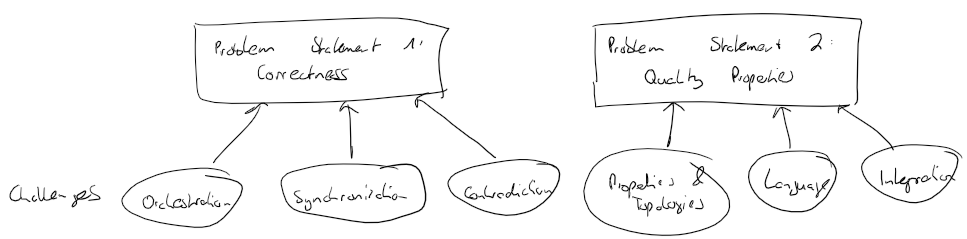
\includegraphics[width=\textwidth]{figures/prologue/challenges.png}
    \caption[Problem statements and challenges]{The two central identified problem statements and challenges identified for them}
    \label{fig:prologue:challenges}
\end{figure}

\mnote{Summary of problems statements and challenges}
We have discussed several issues regarding the construction of transformation networks.
We summarize the problem statements and challenges in \autoref{fig:prologue:challenges}.
We made two central problem statements, one regarding the correctness of networks and one regarding the improvement of quality properties.
Each of these problems is driven by three challenges.
We identified orchestration, synchronization and contradiction to be central challenges for constructing \emph{correct} transformation networks.
For the improvement of quality properties, we emphasized that the relation between properties and topologies challenges the identification of a topology to mitigate property trade-offs and to define an appropriate language for that.
To achieve completeness of a network, we identified the integration challenge to integrate all kinds of artifacts into a transformation-based consistency process.



%%
%% RESEARCH OBJECTIVE
%%
\section{Research Objective}

\mnote{Research questions, assumptions and contributions}
We have identified the central problems and specific challenges that we have to deal with when constructing transformation networks.
In the following, we derive our research goal and the actual research questions that we will answer in this thesis from those challenges.
Afterwards, we summarize the context and the assumptions that we make in our work.
Finally, we give an overview of the contributions that we make to answer the defined research questions.

\subsection{Research Goal and Questions}

The central goal of our research can be summarized as follows.
\begin{researchgoal}
Define a notion of correctness for networks of modular, independently developed transformations and classify relevant quality properties.
Provide an approach to systematically improve correctness and quality properties either by construction or by analysis.
\end{researchgoal}

\mnote{Benefits of achieving goal}
The benefits of achieving that goal are twofold.
First, researchers and transformation developers both gain systematic knowledge about how to achieve correctness and improve quality properties in transformation networks.
Second, transformation developers are provided with concrete techniques and languages that help to achieve correctness and improve other properties either by construction or at least by analysis.


% \subsection*{Properties of Transformation Networks}

% Overall Goal: We want to find out which properties are relevant when building transformation networks and how they are affected by different topologies. This is supposed to help finding ways of systematically improving those properties.

% \begin{researchquestions}{1}
% 	\item \researchquestion{rq:properties}{What are relevant properties and topologies of transformation networks and how do they depend?}
% 	\begin{subresearchquestions}
% 		\item \researchquestion{rq:properties:properties}{Which functional and non-functional properties are relevant when defining transformation networks?}
% 		\item \researchquestion{rq:properties:topologies}{How can network topologies be classified regarding the properties identified in \researchquestionref{rq:properties:properties}?}
% 	\end{subresearchquestions}
% \end{researchquestions}

% \begin{enumerate}[label=\itshape RQ \arabic*.]
% 	% Issue classification
% 	\item Which issues can occur when independently developed \acp{BX} are combined to a network?
% 	\begin{nestedenum}
% 		\item Which failures can occur, when \acp{BX} are combined to a network?
% 		\item What mistakes can be made that lead to failures?
% 		\item How can these mistakes be categorized regarding conceptual levels in the specification process for \acp{BX}?
% 	\end{nestedenum}
% 	\item How are properties of transformation networks affected by the topology?
% 	\begin{nestedenum}
% 		\item Which properties are relevant when defining networks of \acp{BX}?
% 		\item Which topologies of network exist and how do they affect that properties?
% 	\end{nestedenum}
% \end{enumerate}

% \subsubsection*{Evaluation}

% Keine dezidierte Evaluation, lediglich Argumentation


\subsubsection*{Building Correct Transformation Networks} % Correctness of Transformation Networks?

\mnote{Correctness questions}
The first part of our research goal concerns correctness of transformation networks.
We want to know what \emph{correctness} means for transformation networks, which aspects of correctness we can achieve for every network, which of them we can be achieved by assumption, i.e., by proper construction of transformations, which can be analyzed and for which we need to deal with potential incorrectness.

\begin{researchquestions}{1}
	\item \researchquestion{rq:correctness}{When should networks of independently developed transformations be considered \emph{correct} and how can correctness be achieved?}
	\begin{subresearchquestions}
		\item \researchquestion{rq:correctness:notions}{What are relevant notions of correctness in transformation networks and how can they be formalized?} % EV: Argumentation
		\item \researchquestion{rq:correctness:compatibility}{When are the constraints induced by transformations contradictory and how can that be analyzed?} % EV: Proof and empirical application in case study
		\item \researchquestion{rq:correctness:synchronization}{Which requirements must an individual transformation fulfill for being used in a network in comparison to using it on its own?} % EV: Proof and empirical application in case study
		\item \researchquestion{rq:correctness:orchestration}{How can transformations in a network be orchestrated and which properties can such an orchestration strategy fulfill?} % EV: Argumentation, Examples
		\item \researchquestion{rq:correctness:errors}{Which errors can occur in transformation networks, how can they be classified regarding their avoidability and how severe are they?} % EV: Case Study
	\end{subresearchquestions}
\end{researchquestions}

\mnote{Relation between question and challenges}
\researchquestionref{rq:correctness:notions} is the fundamental question to precisely define what \emph{correctness} means, beyond our yet informally given notion.
\researchquestionref{rq:correctness:compatibility}, \researchquestionref{rq:correctness:synchronization} and \researchquestionref{rq:correctness:orchestration} directly map to the previously identified challenges regarding orchestration, synchronization and contradiction.
Finally, \researchquestionref{rq:correctness:errors} asks for the inverse, i.e., for the case when errors occur due to incorrectness, to find out how incorrectness manifests and how severe it is.


% \begin{enumerate}[label=\itshape RQ \arabic*.]
% 	\setcounter{enumi}{2}
	% % Contradiction analysis
	% \item How can transformations be analyzed regarding contradictions in specified constraints?
	% \begin{nestedenum}
	% 	\item What is an appropriate formalism for describing transformations that can be analyzed regarding potential contradictions?
	% 	\item Which kinds of contradictions can be detected by analyzing transformations following a specific formalism?
	% \end{nestedenum}
	% % Issue avoidance by construction
	% \item How can interoperability of independently developed \acp{BX} be achieved by construction?
	% \begin{nestedenum}
	% 	\item Which kinds of mistakes can be avoided by construction of the individual \acp{BX}?
	% 	\item How can we prove that those mistakes and only those mistakes can be avoided by construction?
	% 	\item How can each of these mistakes be avoided by a transformation developer during independent development of a single \acp{BX}?
	% \end{nestedenum}
	% % Orchestration
	% \item What is an appropriate strategy for orchestrating independently developed \acp{BX} to perform a fixed-point iteration?
	% \begin{nestedenum}
	% 	\item Which strategies for orchestrating a network of \acp{BX} exists and what are their properties?
	% 	\item How should those properties be weighted and which of the strategies should be chosen for orchestration?
	% \end{nestedenum}
% \end{enumerate}

% \subsubsection*{Evaluation}

% \gqm{Functionality}{The analysis can be used to find contradictions in specifications}
% {Does the analysis find contradictions if they exist?}
% {Recall: Ratio of true positives to true positives + false negatives}
% \qm{Does the analysis find contradictions although they do not exist?}
% {Precision: Ratio of true positives to true+false positives}
% \qm{Does the analysis find non-contradictions although they exist?}
% {Ratio of false negatives to false+true negatives}

% \gqm{Functionality}{The techniques to avoid mistakes by construction actually avoid interoperabililty issues}
% {Are the identified failures that can occur complete?}
% {Ratio of number of identified failures to total number of failures}
% \qm{Are the relations of identified mistakes to identified failures correct?}
% {Ratio of failures resolved by fixing the identified mistake to all failures}
% \qm{Does the application of avoidance techniques lead to interoperable transformations?}
% {Ratio of changes that are propagated correctly to those that are not propagated correctly}

% \gqm{Applicability}{The techniques can be applied independently to single transformations}
% {Are there cases in which information about other transformations are necessary to solve issues?}
% {Ratio of number of fixes that require information about other transformation to total number of fixes with user interactions\\
% Ratio of number of fixes that require information about other transformation to total number of fixes without user interactions}


\subsubsection*{Improving Quality Properties of Transformation Networks}

\mnote{Quality properties questions}
The second part of our research goal concerns quality properties of transformation networks.
We want to known how we can systematically improve the quality of transformation networks. We want to find out which properties are relevant when building transformation networks and how they are affected by different topologies. 
We use this to systematically derive a proper construction approach achieving a specific topology that resolves trade-offs between quality properties. 
%Second, by including models that were not explicitly modelled as such before to allow their integration into a transformation-based consistency process.

\begin{researchquestions}{2}
	\item \researchquestion{rq:quality}{How can quality properties of transformation networks be systematically improved?}
    \begin{subresearchquestions}
        \item \researchquestion{rq:quality:properties}{What are relevant properties and topologies of transformation networks?} % EV: Argumentation
		\item \researchquestion{rq:quality:topology}{How can topologies of transformation networks improve quality properties of transformation networks?} % EV: Argumentation
		\item \researchquestion{rq:quality:language}{How can a specialized language support the specification of a network topology that improves quality properties?} % EV: Proof-of-concept and case study
		\item \researchquestion{rq:quality:process}{How can software development artifacts be integrated into a transformation-based consistency process?} % EV: Case study
	\end{subresearchquestions}
\end{researchquestions}

\mnote{Relation between question and challenges}
\researchquestionref{rq:quality:properties} and \researchquestionref{rq:quality:topology} directly map to the properties and topologies challenge for identifying how topologies affect properties and how to use them for improving quality properties.
\researchquestionref{rq:quality:language} then maps to the language challenge for designing an appropriate language that supports the construction of an appropriate topology.
Finally, \researchquestionref{rq:quality:process} maps to the integration challenge for lifting artifacts to models that can be used in a transformation-based consistency process.

% \begin{enumerate}[label=\itshape RQ \arabic*.]
% 	\setcounter{enumi}{5}
% 	\item How can a topology of transformation be build that optimizes non-functional properties of transformation networks?
% 	\begin{nestedenum}
% 	    \item How can transformation contradictions be avoided by language design? %uniqueness of consistency specification and consistency among themselves achieved by language design?
% 	    \item How can modularity be achieved in a way such that an arbitrary set of metamodels for which consistency is specified can be used in an actual project?
% 	\end{nestedenum}
% 	% Building tree topologies
% 	\item How should a language specific for multi-model consistency be defined that supports a non-functional property-optimizing topology definition?
% 	\begin{nestedenum}
% 		\item What are the design decisions for such a language?
% 	\end{nestedenum}
% \end{enumerate}

% \subsubsection*{Evaluation}

% \gqm{Functionality}{Concept and language can achieve consistency between several models}{How many model changes in a case study can be properly kept consistent?}{Ratio of successfull test cases}

% \gqm{Practicality}{The assumption of defining a tree of \commonalities is achievable in practice}{Is the definition of cross-tree relations necessary in a case study?}{Number of cross-tree relations in a case study compared to number of relations}

% \gqm{Practicality/Benefit}{A specific language improves conciseness of consistency specifications}{How much more concise is the specification for a case study compared to a definition with direct transformations?}{Number of SLOC with \commonalities compared to number of SLOC with \reactions for same case study}

% Diskussion: Erreichen der Modularität auch evaluieren? Ist per Konstruktion gegeben, könnte man aber natürlich auch noch auswerten (bringt aber nichts).



%% CONTEXT AND ASSUMPTION
\subsection{Context and Assumptions}
\label{chap:introduction:objective:assumptions}

\mnote{Model-driven processes}
In this thesis, we consider the context of model-driven development processes, be it software or software-intensive technical systems.
Thus, we assume that the system under construction is described by several models containing information about different extract or properties of the systems.
We assume that they usually share some overlap of information.
Our discussions will be focus on software development artifacts.
As long as the follow the same formalisms, however, the insights and techniques may be applied to artifacts from arbitrary domain.

\mnote{Distributed knowledge and independent development}
We assume that the knowledge about different transformations to be combined to a network is distributed.
To foster the development of transformations that can be used as \gls{COTS}, we assume that transformations are developed independently.
Thus, transformations may not be adapted to achieve to solve certain issues.

\mnote{No restriction in consistency relation types}
We do not restrict the kinds of relations between models to keep consistent  in any way.
We will, however, discuss in \autoref{chap:networks:notions:types} different types of consistency and their relations to different kinds of processes to preserve consistency.
In fact, our contributions, although theoretically not restricted to that, will be best applicable to a kind of \emph{structural} dependencies rather than \emph{behavioral} dependencies.

\mnote{No consideration of semi-automatism}
Finally, transformations may not always be able to restore consistency on their own, because information to do so is missing.
Consider the case that a developer introduces a class in Java and the transformation has to decide whether that class shall represent a component in \gls{PCM} or not.
That problem can either be solved by requiring the class to fulfill certain patterns, like containing \enquote{Component} in the class name, or by asking the user about his intent.
In cases where information is transformed to a semantically richer models, often further information about how to transform is necessary.
In this thesis, however, we do assume that consistency is preserved automatically, thus excluding the semi-automatic case.
We will finally discuss how our finding generalize to the case where user decisions need to be included.

% Focus on development, rather than usage -> motivate comprehensibility with developer, not with user


%% CONTRIBUTIONS
\subsection{Contributions}

\begin{figure}
    \centering
    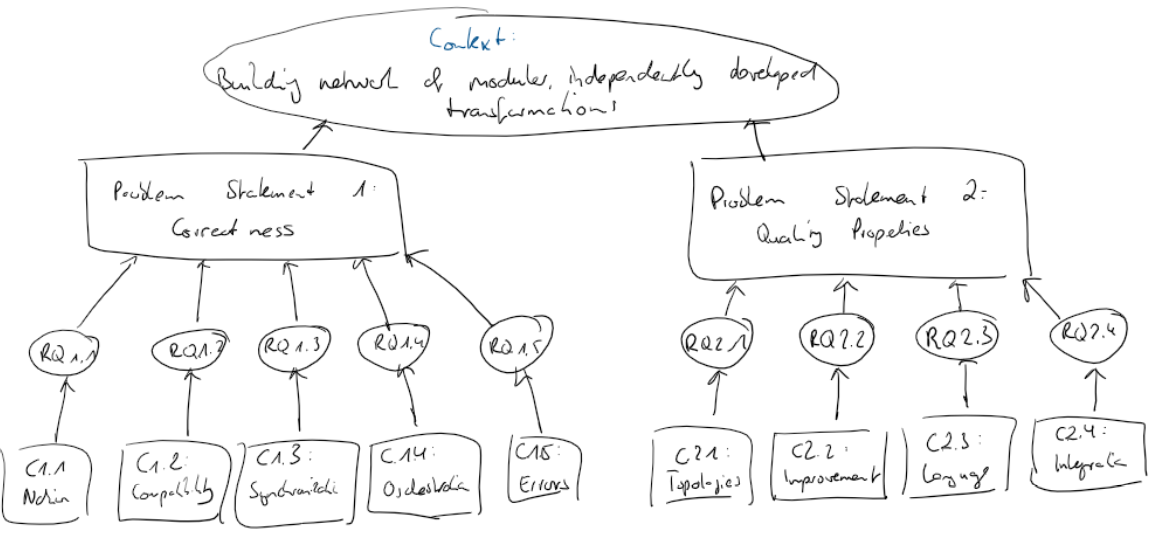
\includegraphics[width=\textwidth]{figures/prologue/context_problem_eq_contribution_relations.png}
    \caption[Context, problems, research questions and contributions]{Relation between context, problem statements, research questions and contributions}
    \label{fig:prologue:context_problem_eq_contribution_relations}
\end{figure}

\mnote{Contribution structure}
The contributions that we make in this thesis are structured along the same dimensions as the problems and the research questions, namely correctness and quality properties.
The contributions directly map to the research questions.
\autoref{fig:prologue:context_problem_eq_contribution_relations} gives an overview of the relations between the problem statements, the research questions and the contributions that we make.

We make the following contributions regarding transformation network correctness:

\begin{contributions}{1}
    \contribution{contrib:correctness:notion}{Notion}{We discuss different notions of correctness for transformation networks and precisely define the one relevant for our context. We derive that compatibility, synchronization and orchestration constitute the relevant correctness notions.}
    \contribution{contrib:correctness:compatibility}{Compatibility}{We precisely define a notion of compatibility to express when transformation contain contradictory constraints. We propose an approach that validated compatibility of transformations which is proven correct.}
    \contribution{contrib:correctness:synchronization}{Synchronization}{We discuss how synchronization can be achieved for transformation defined with existing transformation languages. We make a case distiction over all possible synchronization cases to derive a complete list of problematic synchronization cases. We define a strategy to solve each of them by construction.}
    \contribution{contrib:correctness:orchestration}{Ochestration}{We prove that transformation, in general, can neither be executed only once nor an arbitrary number of times in a fixed-point iteration without the risk of non-termination and thus a strategy must operate conservatively. We discuss why we cannot make restrictions to the transformations to achieve decidability of terminating orchestrations. We propose an orchestration strategy that helpts to find the cause in cases when no orchestration that delivers consistent models is found.}
    \contribution{contrib:correctness:errors}{Errors}{We systematically derive which errors can occur when correctness of a transformation network is not given. We also empirically evaluate the probability of occurance for the errors to classify their severity.}
\end{contributions}

We make the following contributions regarding the improvement of quality properties of transformation networks:

\begin{contributions}{2}
    \contribution{contrib:quality:topologies}{Topologies}{We discuss how different quality properties of transformation networks are affected by the network topology. We derive that trade-off decisions have to be made between the improvement of different properties.}
    \contribution{contrib:quality:improvement}{Improvement}{We propose a strategy for building a specific network topology based on auxiliary models, which make the consistency relations explicit in terms of models rather than transformation. We show that this approach systematically improves different quality properties and mitigates necessary trade-off decisions.}
    \contribution{contrib:quality:language}{Language}{We propose a specialized language for the definition of a network according to the stratefy of %\contributionref{contrib:quality:improvement}. 
    We discuss different design options for the language and its operationalization.}
    \contribution{contrib:quality:integration}{Integration}{We propose an approach for lifting existing models, which are only implicitly encoded in code, to an explicit representation according to a modelling formalism. It enables the usage of implicit models in a model-driven development process.}
\end{contributions}


\subsection{Benefits}

\mnote{Benefits for researchers, transformation (network) developers, and users}
The contributions we make in this thesis provide several benefits to researchers, developers of transformations and transformation networks, as well as transformation (network) users.
All of them profit from systematic knowledge about what \emph{correctness} means for transformation networks, how correctness is affected and can be guaranteed, and about relevant \emph{quality properties} in transformation networks as well as how they can be improved.
The contributions, however, have an intended focus on supporting transformation and transformation network developers. 

\mnote{Benefits for researchers}
Researchers can base on our definitions for correctness of transformation networks and can thus precisely contribute to particular parts of the defined correctness notions, e.g., by approaches to achieve correctness, with explicitly knowing how and which kinds of potential errors of transformation networks are affected by that.
Additionally, they can base further research on the insights about trade-offs between quality properties induced by different network topologies.

\mnote{Benefits for transformation (network) developers}
The developers of actual transformation networks can be separated in the developers of the individual transformations and the ones combining them to a network.
The development of individual transformations is supported by the provision of systematic approaches to build transformations that can be used in networks, especially in terms of supporting synchronization.
Transformation network developers benefits from the knowledge that they have to deal with conservativeness of transformation orchestration.
They also benefit from approaches to validate transformations they want to combine regarding compatibility, an actual and practical orchestration strategy to execute transformations and an approach to build networks that mitigate trade-offs between quality properties.

\mnote{Benefits for transformation (network) users}
Finally, the users of a transformation network, i.e., the ones who develop a system using a transformation network to preserve consistency of their artifacts, benefit from the ability to use networks, for which correctness was systematically achieved, at all.
They also profit from an orchestration strategy that supports them in finding and understanding the reasons why the networks may not be able to process certain changes to preserve consistency.



%%
%% OUTLINE
%%
\section{Thesis Outline}

\todo{Write outline}

First some general considerations, notation, formal basis etc.

Structured along correctness / quality properties
Each chapter maps to one of the defined contributions

Reading process: Correctness and quality properties are almost independent, so possible to start with any of the parts. Within the parts, consecutive reading recommended.
However:
Correctness: Start with notion chapter, then proceed with any of the following, no strict dependencies
Quality (read first chapter of correctness first): First three chapters depend on each, so do not jump. Fourth chapter (integration) is independent.




%%
%% OLD: COPIED FROM PAPERS
%%

%\begin{copiedFrom}{DocSym}

%\section{From DocSym}
%\todo{Clearly introduce running example, removed from content section!}
%\todo{Introduce set notation, say that is it not practically applicable and a strong simplification, but just used to illustrate the problems and solution approaches} % Done at the end
%\todo{Introduce transitive operator R1 o R2 = (R1 u R2) * $\backslash$ (R1 u R2)} % Done at the end

%\todoConference{The problem the research intends to solve, the target audience of this research, and a motivation of why the problem is important and needs to be solved.}

%\acl{MDSD} proposes the usage of models as primary artifacts of the %software 
%development process~\cite{stahl2006a}. 
%Those models describe different system properties for the interests of specific stakeholders, known as \emph{multi-view modelling}, or at different abstraction levels, representing refinements. In both cases, the models describe the same system and are thus not disjoint but contain redundant or dependent information. 
%\todoErik{Wieder: Die beschreiben ja keine Abstraktion, die sind eine Abstraktion. \enquote{Domains of the system} klingt auch komisch, ich weiß zwar, was Du meinst, aber nenne es nicht \enquote{domain}, sondern lieber \enquote{properties}}
%Developers must be aware of those dependencies to ensure that models are modified consistently. 
%Otherwise, the deployed software, which is derived from those models, will potentially not operate correctly.
%\todoErik{Lenkt den Fokus etwas zu stark auf Korrektheit, die wir nicht formal beweisen. Es geht ja nicht nur darum, daß die Software nicht korrekt arbeitet -- möglicherweise tut sie das ja, obwohl die Modelle inkonsistent sind, und das Problem tritt erst bei der Wartung/Evolution auf.}

%In large software systems, a single developer cannot know about all dependencies~\cite{petrenko2008a}, %which can be formulated as \emph{consistency constraints} and 
%in the following referred to as \emph{consistency relations}, which inevitably leads to inconsistencies. 
%Therefore, automated mechanisms that preserve consistency according to those consistency relations are necessary. 
%For that purpose, incremental, bidirectional model transformations %or specialized model synchronization approaches 
%are commonly used. However, most research considers \emph{binary transformations}, restricted to pairs of models, and does not explicitly consider consistency between more than two models~\cite{stevens2017a}, which we refer to as \emph{multi-model consistency}.
%In general, keeping more than two models consistent is currently not researched well.
%Model transformations can either be specified imperatively or declaratively. They differ in who operationalizes the preservation of constraints that have to hold, in the first case the transformation developer and in the second case an automated mechanism of the transformation language. This is why we do not explicitly distinguish these approaches, as all problems apply to both approaches and only different roles have to deal with them. 
% Model transformations can either be specified imperatively, such that the transformation developer has to define how to react to a change, or declaratively, such that the transformation developers only the constraints that have to hold and an automated mechanism derives an imperative operationalization from that.
% We will not explicitly distinguish these approaches, as the identified problems and our solution proposals apply to both. The only difference is that in imperative approaches the transformation developer has to deal with them and in declarative approaches the developer of the transformation language has to consider them when defining the generation of the operationalization.

% Although it is possible to combine binary transformations by transitively executing them, it is yet unclear what problems may arise from that, especially if each transformation is developed independently and treated as a black box.
% We will exemplify this on the simple example in \autoref{fig:prologue:binary_combination_example}, in which consistency relations define a mapping of a component in an \ac{ADL} to a class in object-oriented design, which is again represented by an implemented class in Java code. 
% The name of the class is defined to be the component name with an \enquote{Impl} suffix (cf.~\cite{langhammer2017a}).
% When all these relations are expressed in transformations, it is, for example, possible that both transformations from \ac{ADL} to Java, once over \ac{UML} (\ref{fig:prologue:binary_combination_example:R1} and \ref{fig:prologue:binary_combination_example:R2}) and once directly (\ref{fig:prologue:binary_combination_example:R3}), create a Java class after creating an \ac{ADL} component.
% We refer to that as an \emph{interoperability problem}.
% The transformation specification %or its execution engine 
% would have to avoid an overwrite and therefore have to consider dependencies between transformations, using, for example, a shared trace model.
% In general, an interoperability problem is an unexpected behavior of transformations, which only occurs if they are executed transitively, but not if each is executed on its own. %, although all preserve the same consistency relations.

% Additionally, it is easy to see that %specifying multi-model consistency with combinations of 
% combining binary transformations leads to trade-off decisions.
% The ternary relation %between the three metamodels 
% can either be expressed by three binary transformations between all pairs of metamodels or by two binary transformations with the third being %expressed by the transitive 
% the combination of the two others.
% The first option leads to redundancies in the specifications, as each pair of transformations has to have an equal semantics than the third.
% For example, the \ac{ADL} to Java transformation for \ref{fig:prologue:binary_combination_example:R3} must be equal to the combination of the transformations \ac{ADL} to \ac{UML}~(\ref{fig:prologue:binary_combination_example:R1}) and \ac{UML} to Java~(\ref{fig:prologue:binary_combination_example:R2}).
% Consequently, those transformations may be incompatible if not correctly defined, e.g., by leaving out the suffix addition in the transformation for \ref{fig:prologue:binary_combination_example:R3}.
% %As an alternative, the second option is express the ternary relation with two binary consistency relation specifications.
% %For example, specification \ref{fig:example:R3} can be interpreted as a combination of \ref{fig:example:R1} and \ref{fig:example:R2}.
% An alternative is to omit the transformation for \ref{fig:prologue:binary_combination_example:R3} by transitively executing the two others.
% However, in this case, modularity is reduced, because it is not possible to use only Java and the \ac{ADL} to develop a specific system and omit the \ac{UML}.
% %Additionally, comprehensibility decreases, because the relation between \ac{ADL} and Java is only expressed transitively. 
% %This becomes more problematic if transformation paths have a length higher than two.
% We refer to this as \emph{specification trade-offs}.

% \begin{figure}
%     \centering
%     \begin{tikzpicture}

    \node[uml class, align=center, minimum width=10em] (component) {\umlcomponentlabel\\[-0.3em] \small PaymentSystem};
    \node[above=0em of component.north, anchor=south] (adl_label) {\textit{ADL}};
    
    \node[uml class, minimum width=10em, below left=2.15em and 7.5em of component.south, anchor=north, font=\small] (uml_class) {PaymentSystemImpl};
    \node[above right=0em and 1em of uml_class.north west, anchor=south west] (uml_label) {\textit{UML}};
    
    \node[draw, minimum width=10em, below right=2.15em and 7.5em of component.south, align=left, anchor=north, font=\small] (java_class) {
    \textbf{class} PaymentSystemImpl \{ \\[-0.3em]
        \hspace{1em} {\tiny // \ldots} \\[-0.3em]
    \}
    };
    \node[above left=0em and 1em of java_class.north east, anchor=south east] (java_label) {\textit{Java}};
    
    \draw[latex-latex, dashed, thick=false] (component) -- node[above left=-0.5em and 0.5em] {\mylabel{fig:prologue:binary_combination_example:R1}{$R_1$}} (uml_class);
    \draw[latex-latex, dashed, thick=false] ([yshift=-1.5em]uml_class.north east) -- node[above] {\mylabel{fig:prologue:binary_combination_example:R2}{$R_2$}} ([yshift=-1.5em]java_class.north west);
    \draw[latex-latex, dashed, thick=false] (component) -- node[above right=-0.5em and 0.5em] {\mylabel{fig:prologue:binary_combination_example:R3}{$R_3$}} (java_class);
    
\end{tikzpicture}
%     \caption{Example models with binary consistency relations}
%     \label{fig:prologue:binary_combination_example}
% \end{figure}

%Although specific approaches for expressing multiary relations, rather than using combinations of binary relations, could be developed, there are some reasons for adhering to binary transformations.
%Instead of developing approaches to express multiary consistency relations, there are reasons to adhere to binary transformations, and to research their combinability.
%As stated by \textcite{stevens2017a}, %there are especially strong practical reasons, as 
%it is hard enough to think about binary relations. %between pairs of models.
%Defining multiary relations would require a knowledge about the relations between all metamodels used to describe a system.
%Additionally, each domain expert, who specifies transformations, %in practice, 
%will usually only have knowledge about the relations between two or at most a rather limited set of metamodels. %, but not of all involved metamodels. %, which would be necessary to define multiary relations.
%Thus, it is a natural goal to make the modular specification of consistency based on binary transformations possible.
%In the proposed thesis, 
%We therefore plan to make the following contributions to research on multi-model consistency preservation:
%\todoErik{Ich fänd's cool, wenn die Probleme auch irgendwie hervorgehoben sind, und Du die Beiträge schon auf die Probleme beziehen kannst, also Mini-PIBA für jedes Deiner identifizierten Probleme. Würde aber erst die Probleme formulieren, dann den IBA-Teil so wie unten (wobei bei manchen noch die Beschreibung des Benefits fehlt).}
% \begin{description}[leftmargin=\parindent]
%     \item[Transformation interoperability.] %Under the assumption that 
%         When several binary transformations are developed independently, they must be combinable in a black box manner, introduced as the \emph{interoperability problem}. We will therefore identify problems that can arise from that combination %of transformations 
%         and develop a catalog of patters that can be followed by the transformation developer or language to achieve \emph{non-intrusive} interoperability of binary transformations.
%     \item[Decomposition of consistency relations.] 
%         The usage of binary transformations for multi-model consistency preservation leads to \emph{specification trade-offs} regarding essential challenges. We will provide a classification of those challenges and investigate the influence of the way in which transformations are specified on them.
%         %Decomposing the underlying consistency relations into independent sub-relations allows a partial optimization regarding those challenges.
%         %We will therefore investigate how consistency relations can be decomposed into independent subsets.
%         We will especially investigate how consistency relations can be decomposed into independent subsets, as this allows a partial optimization regarding those challenges.
%     %We will identify relevant properties of consistency specifications, which have to be considered when defining those specifications as they introduce trade-off decision. We already motivated some of those properties above and give a more detailed overview in \autoref{sec:multimodelconsistency}.
%     \item[Make common concepts explicit.] 
%         Metamodels often represent the same concepts in different ways. As another contribution to reduce \emph{specification trade-offs}, we propose an approach to make these common concepts explicit to improve comprehensibility of transformations and to improve their modular reuse.
% \end{description}

% We propose an approach for multi-model consistency based on \aclp{VOMM}. 
% In those virtual metamodels, dependencies between metamodels, which we refer to as \emph{consistency relations}, are made explicit by representing common concepts, whereas in model transformations, which we refer to as \emph{consistency preservation specifications}, they are specified implicitly. 
% The envisioned benefit is an inversion of the above mentioned properties. 

%Throughout this paper, we use a simplified notation for metamodels and heir consistency relations to ease their illustration. 
%We consider metamodels to be sets of elements and consistency relations to be sets of symmetric, binary relations between those elements.
%To ease the representation of combinations of consistency relations, we define the concatenation operation for two consistency relations $R_1$ and $R_2$ as:
%\begin{equation*}
%    R_1 \concat R_2 \coloneqq \{(x,y)\, |\, \exists t: x\, R_1\, t\, R_2\, y \}.
%\end{equation*}
%This is the subset of the transitive closure of two relations that contains only the relations transitively defined over $R_1$ and $R_2$.
%It can be also expressed as the natural join of $R_1$ and $R_2$ with an additional projection that removes the common elements of both relations.
%The operator is commutative since the relations are assumed symmetric.

% \todoErik{Würd ich bei so einem kurzen Paper weglassen. (Ich würde es auch oft bei langen Papern weglassen. :-))}
% In this paper, we first discuss related work in \autoref{sec:relatedwork}. 
% In \autoref{sec:approach}, we give an overview of our planned contributions by explaining the problems in detail and sketching our solution approaches. %we first discuss interoperability problems arising from the combination of independently developed binary transformations and give an overview on envisioned solution patterns.
% %We then give an introduction to the yet identified challenges inducing trade-off decisions during transformation development.
% %From this, we derive the consideration of consistency relation composition and an approach to make common concepts explicit.
% % We then discuss problems arising from the black-box combination of binary transformations and give an overview on envisioned solution patterns.
% % In \autoref{sec:vomms}, we introduce our approach to make overlaps of metamodels explicit to improve properties of multiary consistency specifications.
% Finally, we discuss the current state and planned evaluation in \autoref{sec:status} and conclude the paper in \autoref{sec:conclusion}.


% \begin{itemize}
%     \item Motivation MDSD
%     \item Several models describe single system
%     \item Information overlap between models, e.g. component architecture and code, ref to Michael
%     \item Developers must be aware of redundancies and dependencies, otherwise inconsistencies
%     \item Best: Make redundancies/dependencies explicit for (semi-)automated mechanisms for preserving consistency
%     \item Incremental model transformations can be used (refs) or specialized model consistency or model synchronization approaches (refs)
%     \item Existing approaches only concern consistency preservation between instances of two metamodels
%     \item If more than two models are involved, these approach would require that consistency preservation is executed transitively
%     \item From that, problems arise
%     \begin{itemize}
%         \item Inconsistent consistency specifications: Consistency specifications between different metamodels must be consistent. E.g. having 3 metamodels, a consistency specification between two of them can be contradictory to the two other
%         \item Consequence: Result of a modification depends on the order in which consistency specification are evaluated or even results in propagation cycle due to alternating changes -- EXAMPLE
%         \item Ordering problem: Preserving consistency after a change can require several changes in other models. The order in which they are executed can produce different results -- EXAMPLE
%         \item Confluence problem: Changes can be propagated across several paths, if more than two models are involved. This can result in conflicts, if the propagation confluences in one model. E.g. it can be necessary to create a metaclass instance in that model to preserve consistency. All confluencing change propagations require the creation of an element, but how can you achieve that only the first one creates it and the other see the new element and reference it instead?
%     \end{itemize}
% \end{itemize}

%\todoHeiko{Define metamodel vs. \modelinglanguage, Use \modelinglanguage or DSL?}
%\todoHeiko{Say: code is also a model}
%\todoHeiko{Define: \emph{consistency relation} for existing relationships between metamodels that require consistency preservation and \emph{consistency preservation specification} for mechanisms that semi-automatically preserve consistency according to an existing consistency relation}
%\todoHeiko{We refer to the process of preserving consistency due to defined consistency preservation specifications as \emph{change propagation}, as a performed change resulting in the violation of consistency relations leads is propagated to restore consistency -- Besser change propagation überall weglassen.}
%\todoHeiko{Introduce trace links and their necessity for identifying corresponding elements according to consistency relations (prescriptive vs. descriptive)}


%\todo{Klarmachen, dass es immer darum geht Konsistenzrelationen durch bidirektionale, binäre Transformationen auszudrücken. Das ist die Baseline.}

%\todo{Klarmachen, dass Kombination binärer Transformationen der state-of-the-art ist.}

%\end{copiedFrom} % DocSym


% \begin{copiedFrom}{SoSym MPM4CPS}

% \section{From SoSym MPM4CPS}

%%
%% Scope: Building large systems of many models
%%
%The scale of modern software systems and their embedding into cyber-physical systems leads to a high and even increasing complexity of systems to be built. 
%To handle that complexity, different roles operate on appropriate extracts and abstractions of the system under construction described by different models or views.
%Such a fragmentation of information across different models is common at a high level, i.e., mechanical, electrical and software engineers usually use different models and associated tools to describe a system in their domain.
%Additionally, different models can be used on a low level by engineers from the same domain, such as software engineers using different models for architecture specification, behavior development and deployment.
%For example, the development of \acp{ECU} software in automotives comprises different tools or standards for specifying the system and software architecture, such as SysML~\cite{sysml} or AUTOSAR~\cite{scheid2015autosar}, for defining the behavior, such as MATLAB/Simulink~\cite{simulink} or ASCET~\cite{ascet}, and for defining the deployment on multi-core hardware architectures, such as Amalthea~\cite{amalthea, wolff2014a}.
%Since all these models describe the same system, they usually share an overlap of information in terms of dependencies or redundancies, which can lead to inconsistencies if overlapping information is not modified properly in all models.
%Recent research investigated such dependencies between ASCET and SysML~\cite{giese2010a}, as well as Amalthea and how to resolve them~\cite{mazkatli2017ase,mazkatli2016ma}.

%%
%% General solution: incremental BX combined to a network
%%
%For resolving inconsistencies, different approaches have been developed.
%Incremental model transformations are a common approach to resolve such inconsistencies by enabling developers to explicitly specify how inconsistencies can be resolved (semi-)automatically. 
%Especially bidirectional model transformations~\cite{stevens2010sosym}, which specify the relations between two metamodels and routines how consistency of their instances can be restored, are well suited and well researched.
%Relating more than two metamodels can either be achieved by defining a multi-directional transformation between all of them or by specifying bidirectional transformations %transformations between pairs of metamodels, i.e., bidirectional transformations, 
%between pairs of them in a modular way and combine them to a network that is able to check and preserve consistency between several models.
%In consequence, a more reasonable option is to specify transformations between pairs of metamodels, i.e., bidirectional transformations, in a modular way and combine them to a network that is able to check and preserve consistency between several models.
%\begin{example}
% \autoref{fig:prologue:three_persons_example} exemplifies these different possibilities at the example of relation of transformations between three simple metamodels for persons, employees and residents.
% We use an informal notion of consistency, defined more precisely later on, which requires that if any person, employee or resident is contained in a model, there must also be the other two elements with the same names, addresses, incomes and social security numbers. %fulfilling a specific relation of their properties.
% %That relation includes that names, addresses, incomes and the social security numbers % (\texttt{socsecnumber}) 
% are equal.
% This relation can either be expressed as a ternary relation, denoted as $R_{PER}$, or as three binary relations $R_{PE}, R_{PR}, R_{ER}$.
% In such a simple scenario a single developer may be able to define all these relations.
% However, in a more complex scenarios, like the relations between the previously mentioned SysML, Amalthea and ASCET metamodels, there may not be a single person having the knowledge about all these dependencies~\cite{petrenko2008a}, but there may be different domain experts knowing about relations between subsets of the metamodels~\cite{klare2018docsym}.
% Additionally, it is difficult to think about complex multiary relations~\cite{stevens2017a}.
% In consequence, building networks of bidirectional transformations provides several benefits over building multi-directional transformations.
% %\end{example}

% \begin{figure}
%     \centering
%     %% From motivational_example in MPM4CPS paper

\newcommand{\hdistance}{10.6em}
\newcommand{\classwidth}{6em}

\begin{tikzpicture}

% Person
\umlclassvarwidth{person}{}{Person\sameheight}{
firstname\\
lastname\\
address\\
income
}{\classwidth}

% Employee
\umlclassvarwidth[,above right=3em and \hdistance of person.east, anchor=south]{employee}{}{Employee\sameheight}{
name\\
socsecnumber\\
salary
}{\classwidth}

\umlclassvarwidth[,below=6em of employee.south, anchor=north]{resident}{}{Resident\sameheight}{
name\\
address\\
socsecnumber
}{\classwidth}


% CONSISTENCY RELATIONS
\draw[consistency relation] (person.north) |- node[pos=0, above left] {$p$} node[pos=0.75, above] {$R_{PE}$} node[pos=1, above left] {$e$} (employee.west);
\draw[consistency relation] (employee.south) -- node[pos=0, below right] {$e$} node[right, align=left] {$R_{ER}$ /\\ $R'_{ER}$} node[pos=1, above right] {$r$} (resident.north);
\draw[consistency relation] (resident.west) -| node[pos=0, below left] {$r$} node[pos=0.25, below] {$R_{RP}$} node[pos=1, below left] {$p$} (person.south);

\draw[consistency relation 2] (person.east) -- node[pos=0, below right] {$p$} ++(0.35*\hdistance,0) -- node[pos=0, right=0.5em] {$R_{PER}$} node[pos=1, above left] {$e$} ([yshift=1em]employee.south west);
\draw[consistency relation 2, ->] ([xshift=0.35*\hdistance]person.east) -- node[pos=1, below left] {$r$} ([yshift=-1em]resident.north west);

\node[consistency related element 2, below left=5em and 2.5em of person.south west, anchor=north west] (relations1) {
$\begin{aligned}
    R_{PER} =\; &
            \setted{\tupled{p,e,r} \mid \\
            & p.firstname + "\text{\textvisiblespace}" + p.lastname = e.name = r.name\\
            & \land p.address = r.address%\\
            %& 
            \land p.income = e.salary\\
            & \land e.socsecnumber = r.socsecnumber
        }
\end{aligned}$
};

\node[consistency related element, below=0.5em of relations1.south west, anchor=north west] {
$\begin{aligned}
    R_{PE} =\; &
            \setted{\tupled{p,e} \mid %\\
            %& 
            p.firstname + "\text{\textvisiblespace}" + p.lastname = e.name\\
            & \land p.income = e.salary
        }\\[0.3em]
    R_{PR} =\; &
            \setted{\tupled{p,r} \mid %\\
            %& 
            p.firstname + "\text{\textvisiblespace}" + p.lastname = r.name\\
            & \land p.address = r.address
        }\\[0.3em]
    R_{ER} =\; &
            \setted{\tupled{e,r} \mid %\\
            %& 
            e.name = r.name\\
            & \land e.socsecnumber = r.socsecnumber
        }\\
    R'_{ER} =\; &
            \setted{\tupled{e,r} \mid %\\
            %& 
            e.name.toLower = r.name\\
            & \land e.socsecnumber = r.socsecnumber
        }
\end{aligned}$
};

\end{tikzpicture}
%     % {\color{consistencycolor2}\begin{align*}
%     %     R_{PER} = &
%     %         \setted{\tupled{p,e,r} \mid \\
%     %         & p.firstname + "\text{\textvisiblespace}" + p.lastname = e.name = r.name\\
%     %         & \land p.address = r.address%\\
%     %         %& 
%     %         \land p.income = e.salary\\
%     %         & \land e.socsecnumber = r.socsecnumber
%     %     }
%     % \end{align*}}
%     % \vspace{-2em}
%     % {\color{consistencycolor1}\begin{align*}
%     %     R_{PE} = &
%     %         \setted{\tupled{p,e} \mid %\\
%     %         %& 
%     %         p.firstname + "\text{\textvisiblespace}" + p.lastname = e.name\\
%     %         & \land p.income = e.salary
%     %     }\\
%     %     R_{PR} = &
%     %         \setted{\tupled{p,r} \mid %\\
%     %         %& 
%     %         p.firstname + "\text{\textvisiblespace}" + p.lastname r.name\\
%     %         & \land p.address = r.address
%     %     }\\
%     %     R_{ER} = &
%     %         \setted{\tupled{e,r} \mid %\\
%     %         %& 
%     %         e.name = r.name\\
%     %         & \land e.socsecnumber = r.socsecnumber
%     %     }\\
%     %     R'_{ER} = &
%     %         \setted{\tupled{e,r} \mid %\\
%     %         %& 
%     %         e.name.toLower = r.name\\
%     %         & \land e.socsecnumber = r.socsecnumber
%     %     }
%     % \end{align*}}
%     % \vspace{-1em}
%     \caption{Three simple metamodels for persons, employees and residents, one ternary relation $R_{PRE}$ between them and three binary relations $R_{PE}, R_{PR}, R_{ER}$ for each pair of them, with $R'_{ER}$ as an alternative for $R_{ER}$.}
%     \label{fig:prologue:three_persons_example}
% \end{figure}

% %%
% %% Problem: Cycles
% %%
% Such a network of bidirectional transformations may contain cycles of transformations.
% \autoref{fig:prologue:three_persons_example} exemplifies why it may be unavoidable to have such cycles. 
% There is no pair of binary relations, such that it is equivalent to the ternary relation $R_{PER}$, because each pair of metamodels shares unique information that is not represented in the third one. %, namely address, income and social security number.
% An essential issue with such cycles is that they impose the possibility of defining contradictory constraints, such that the relations cannot be fulfilled at the same time.
% In such a case, the relations are considered \emph{incompatible}.
% Consider the three binary relations $R_{PE}, R_{PR}, R'_{ER}$ in \autoref{fig:prologue:three_persons_example}.
% These relation cannot always be fulfilled, because $R'_{ER}$ requires the resident name to be lowercase, whereas the other relations relate the names as they are and thus allow the lowercase names.
% In consequence, for a resident with a non-lowercase name it is not possible to find a consistent person and employee.
% However, in a transformation network, compatibility of the relations defined by the transformations is a necessary requirement for their repair routines to properly restore consistency~\cite{klare2019icmt}.

% In this article, we focus on the relations of a transformation, which define when two models are considered consistent.
% Compatibility of such relations is a necessary requirement for the repair routines of transformations to properly restore consistency in a transformation network, as shown in \cite{klare2019icmt}.
% Thus, in the following we only consider the relations defined by transformations rather than the repair routines.

% In this article, we consider the relations defined by bidirectional transformations.
% We clarify the notion of \emph{compatibility} of these relations and develop an approach to prove compatibility of relations in a given network of transformations.
% To achieve this, we formally define a notion of consistency, based on fine-grained consistency relations, as well as compatibility.
% Building on this formalism, we are able to derive an inductive, formal approach for proving compatibility of relations by identifying those that are redundant.
% The essential idea is that if consistency relations have a specific kind of tree structure, we are able to show that they are inherently compatible.
% Furthermore, we show that adding redundant relations to such a tree preserves compatibility.
% In consequence, reducing an arbitrary network of relations to a tree by removing redundant relations proves compatibility.
% Finally, we present an operationalized approach based on that formal approach for \qvtr to prove compatibility of a network of \qvtr relations.
% That approach transforms \qvtr relations into first-oder logical formulae and finds redundant relations by applying an SMT solver.
% % We propose an approach that is able to prove that transformations are compatible, on the example of QVT-R. The approach represents the transformation rules as a graph of metamodel elements with consistency relations between them. Its goal is to find an equivalent set of trees of consistency relations, which are compatible due to the inherent absence of cycles. To achieve that, it decomposes the graph into independent subsets and then removes redundant consistency relations within existing cycles. To prove redundancy of a relation, cycles of relations are transformed into logical expressions and evaluated with an SMT solver. 
% More detailed, we make the following contributions:
% \begin{description}[leftmargin=\parindent]
%     \item[\contributionlabel{contrib:formalization}{Compatibility Formalization}{C1}:] We formalize a notion of consistency and precisely define \emph{compatibility} of relations in a network of transformation.
%     \item[\contributionlabel{contrib:formalapproach}{Formal Approach}{C2}:] We define a formal, inductive approach for proving compatibility of relations based on a notion of redundancy and relation trees. % and proving that such trees are compatible and that redundancy preserves compatibility.
%     \item[\contributionlabel{contrib:operationalizedapproach}{Operationalized Approach}{C3}:] We propose an approach that applies the formalism to %transformation languages. %and thus enables proving compatibility of transformations defined in a transformation language. 
%     %We especially discuss the approach application to 
%     \qvtr and show how a translation to logical formulae and the usage of SMT solver can be used to prove compatibility.
%     \item[\contributionlabel{contrib:evaluation}{Applicability Evaluation}{C4}:] While correctness of the approach is given by construction and proven on the formalism, we apply the approach to case studies to show applicability of the approach. 
% \end{description}

%\todoHeiko{Discuss gap between extension notion in formalism and intensional notion in transformation languages.}

% It is, in general, not possible to prove that transformations are incompatible if the language used to describe consistency relations has sufficient expressiveness and is thus undecidable, such as \qvtr.
% On the other hand, it is possible to prove that transformations are compatible.
% Our approach is designed to operate conservatively, thus in cases it claims compatibility, the transformations actually are compatible.
% However, there may be cases in which relations are compatible but the approach is not able to prove that.

% The main benefit that our approach imposes is that it enables domain experts to define transformations independently and %allows them 
% to automatically detect their compatibility both during development as well as afterwards when combining them to a network.
% This relieves them from the necessity to align the transformations with each other a priori and ensuring compatibility manually.
%It also enables them to constantly check compatibility during the development of transformation.
%Finally, even a single developer defining a transformation network that contains cycles may introduce incompatibilities between the transformations.

% \todoDiss{Discuss different benefits / scenarios more clearly, especially second benefit / application scenario: User define relations and wants on-the-fly feedback on compatibility to other existing relations, rather then a posteriori checking}

% \paragraph{Running Example}

% \begin{figure*}
%     \centering
%     \includegraphics[width=\textwidth]{figures/running_example.pdf}
%     \caption{Metamodel extracts for ASCET/ASEM, Amalthea and OO used in automotive ECU development}
%     \label{fig:running_example}
% \end{figure*}

% \begin{itemize}
    % \item multi-paradigm modeling used in automotive domain
    % \item high-level: different domains such as mechanical design, electric design, software, all with different views
    % \item low-level: even on low level different views
    % \item example low-level: development of electronic control units (ECUs) with behavior specification in ASCET/ASEM block diagrams, behavior refinement in OO code (e.g. C++, generated but also manually modified), multi-core deployment specification in Amalthea (tasks/runnables and their deployment to hardware)
    % \item highly simplified relations specified in \autoref{fig:running_example} (aligned with \cite{mazkatli2017ase})
    % \item actual metamodels are much more complex, involving explicit behavior specifications, I/O (method parameters, return values, ports etc.)
% \end{itemize}

% \end{copiedFrom} % SoSym MPM4CP


